\section{Demonstration Interface}
\label{ch:demo}
\subsection{Purpose}
The preceding results are presented as tables and figures. To allow a reader to explore them interactively, a web interface was built that replays the saved predictions against the actual Bitcoin price. The interface does not retrain a model, retrieve live data or generate new predictions. Every quantity it displays is read from files that the pipeline has already produced.

\subsection{Functionality}
Figure~\ref{fig:demo} shows a full-page capture. A control panel at the top sets the period, the model and the prediction set.
\begin{itemize}
\item \textbf{Date selector.} Two date fields and five presets: the test period, the last three or six months, the last year, and all data.
\item \textbf{Model selector.} The majority rule, XGBoost, LSTM A, LSTM B with VADER and LSTM B with FinBERT.
\item \textbf{Prediction set.} The frozen test split (October 2025 to August 2026) or the walk-forward predictions, which cover January 2023 to August 2026.
\item \textbf{Price chart.} The daily close with one marker per day. A triangle pointing up or down gives the prediction for the next day. It is filled when the call was correct and hollow when it was wrong, so the chart does not depend on colour alone. Hovering reveals the close, the predicted direction and probability, the actual outcome and whether the call was right.
\item \textbf{Summary figures.} Accuracy for the chosen dates, shown beside the range that a guessing model would produce, the number of days, and the shares of predicted and actual rises.
\item \textbf{Sentiment chart.} Daily VADER or FinBERT scores for the same dates, with the no-news gap shaded and not hidden.
\item \textbf{Comparison table.} All five models scored on exactly the same days.
\end{itemize}
A banner on every page states that the output is experimental and not financial advice.

\begin{figure}[htbp]\centering
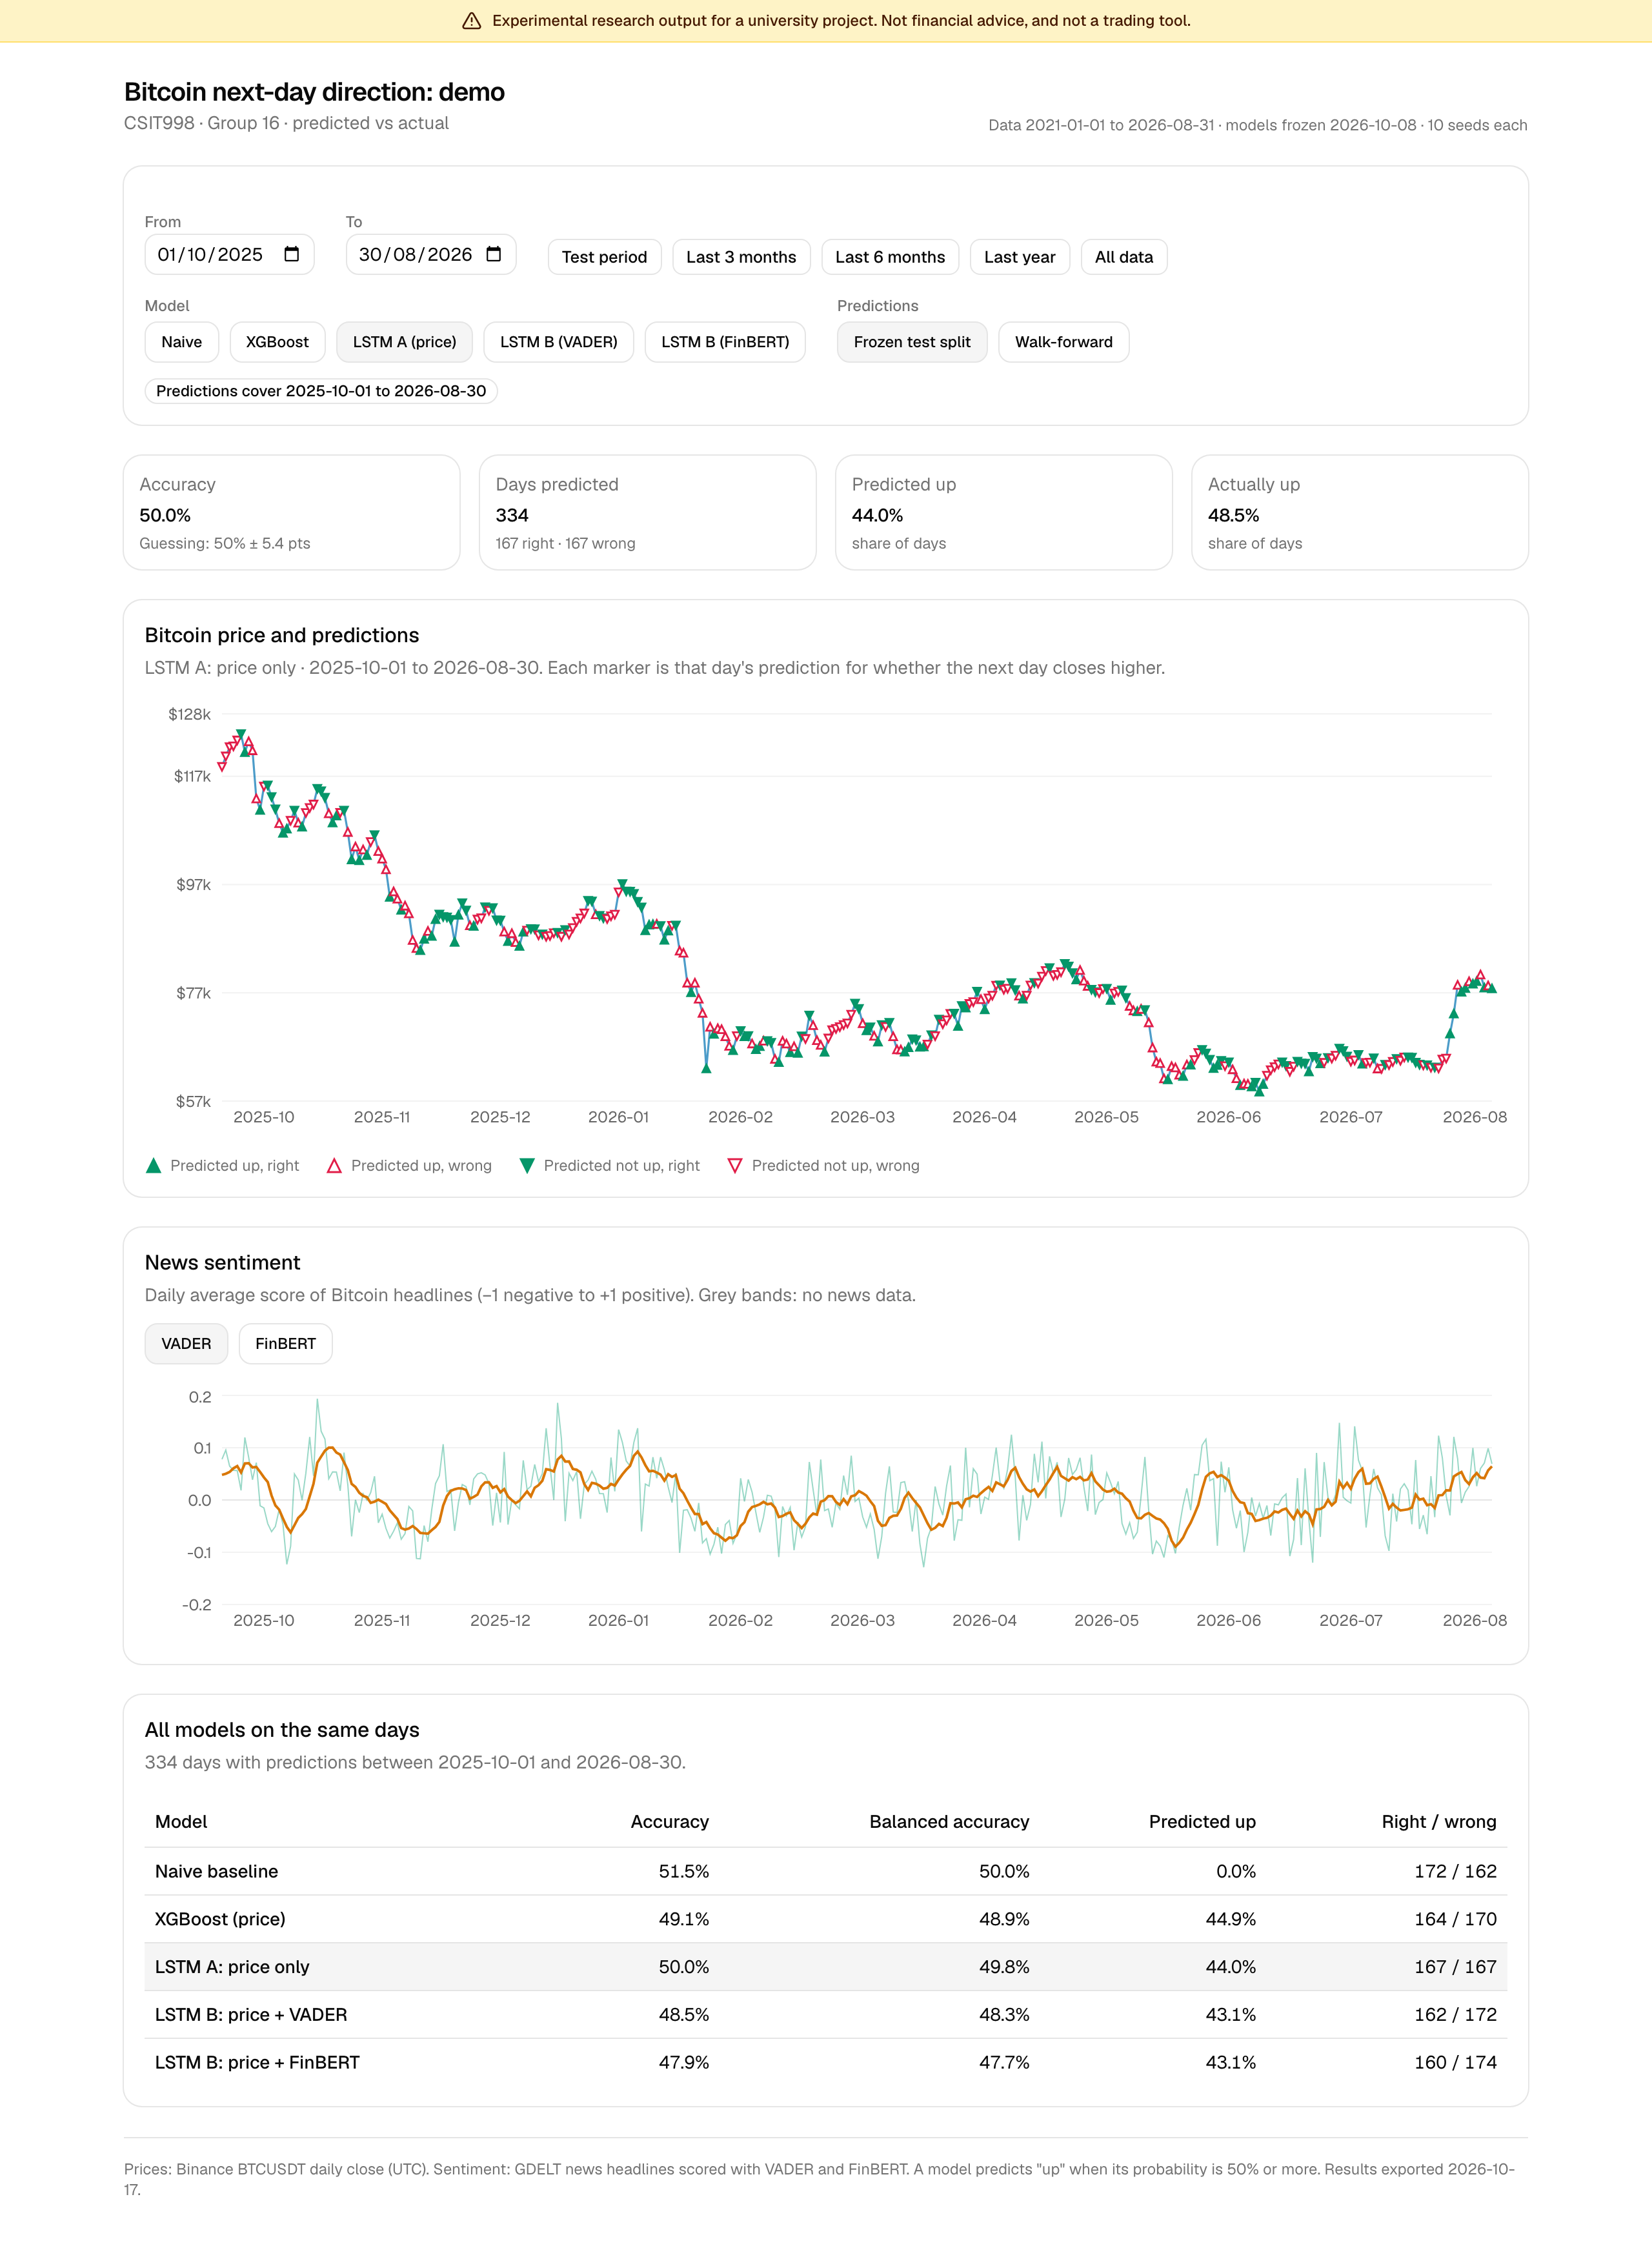
\includegraphics[height=0.78\textheight,keepaspectratio]{figures/demo_interface.png}
\caption{The demonstration interface, showing LSTM A on the frozen test period.}\label{fig:demo}
\end{figure}

\subsection{Implementation}
The interface is a Next.js application written in TypeScript, using Tailwind CSS, shadcn/ui components and the Recharts library, and exported as a static site. It has no server and no database. A Python script, \code{src/export_demo_data.py}, converts the saved results into three JSON files of about 460 KB in total. They hold the daily price and sentiment, each model's saved probability for every day, and a small metadata file. The site is built once from these files and can be hosted on any static service.

Two decisions follow from the governance work in Section~\ref{ch:governance}. The exported files contain only daily aggregates, with no headline text and no article links, and the export script refuses to write either. The page also computes its summary figures in the browser from the saved probabilities, using the same 0.5 threshold as the evaluation. A small test suite verifies this arithmetic together with the date presets.

To run the interface locally, the dependencies in the \code{web/} folder are installed and the development server is started. The README gives the exact commands.

\subsection{Limitations}
The interface replays history. It cannot produce a prediction for tomorrow, and this is deliberate. Given the results in Section~\ref{ch:results}, a live forecast would suggest skill that the evidence does not support. It also displays two prediction sets that were produced under different training schemes, and it labels them so that a viewer does not confuse them.
